%----------------------------------------------------------------------------------------
%	LATEX SAMENVATTING TEMPLATE
%	Versie 1.3 (9 september 2014)
%	Opmerkingen of feedback naar Robert van Wijk
%					(robertvanwijk@uva.nl)
%----------------------------------------------------------------------------------------

%----------------------------------------------------------------------------------------
%	PACKAGES EN DOCUMENT CONFIGURATIE
%----------------------------------------------------------------------------------------

\documentclass[a4paper,12pt]{article}
\usepackage{algorithm2e}
\usepackage[dutch]{babel}
\usepackage{fancyhdr}
\usepackage{graphicx}
\usepackage{hyperref}
\usepackage{lastpage}
\usepackage{longtable}
\usepackage{lipsum}
\usepackage{tabu}
\usepackage{tikz}
	\usetikzlibrary{mindmap,backgrounds}
\usepackage{verbatim}

%----------------------------------------------------------------------------------------
%	DOCUMENT INFORMATIE
%----------------------------------------------------------------------------------------
%Geef bij ieder command het juiste argument voor deze opdracht. Vul het hier in en het komt op meerdere plekken in het document correct te staan.

\newcommand{\opdracht}{Samenvatting}			%Voor deze opdracht niet veranderen
\newcommand{\titel}{Nummer en titel van het hoofdstuk}	%Nummer en titel van het samengevatte hoofdstuk
\newcommand{\studentA}{Naam student}			%Vul je eigen voor- en achternaam in
\newcommand{\uvanetidA}{UvAnetID student}
\newcommand{\tutor}{Naam tutor}				%Vul de voor- en achternaam van je tutor in
\newcommand{\PAVgroep}{Naam  PAV-groep}		%ALGOL (A1), Amiga E (A2), etcetera
\newcommand{\datum}{\today}					%Pas aan als je niet de datum van vanaag wilt hebben

%----------------------------------------------------------------------------------------
%	AUTOMATISCHE HEADER & FOOTER
%----------------------------------------------------------------------------------------
%Hoef je niets aan te veranderen

\pagestyle{fancy}
  \lhead{
\includegraphics[width=7cm]{logoUvA}}		%Zorg dat het logo in dezelfde map staat
  \rhead{\footnotesize \textsc {Samenvatting\\ \titel}}
  \lfoot
    {
	\footnotesize \studentA (\uvanetidA)
    }
  \cfoot{}
  \rfoot{\small \textsc {Pagina \thepage\ van \pageref{LastPage}}}
  \renewcommand{\footrulewidth}{0.5pt}

\fancypagestyle{firststyle}
 {
  \fancyhf{}
   \renewcommand{\headrulewidth}{0pt}
   \chead{
\includegraphics[width=7cm]{logoUvA}}
   \rfoot{\small \textsc {Pagina \thepage\ van \pageref{LastPage}}}
 }

\setlength{\topmargin}{-0.3in}
\setlength{\textheight}{630pt}
\setlength{\headsep}{40pt}

%----------------------------------------------------------------------------------------
%	AUTOMATISCHE TITEL
%----------------------------------------------------------------------------------------
%Hoef je niets aan te veranderen

\begin{document}
\thispagestyle{firststyle}
\begin{center}
	\textsc{\Large \opdracht}\\[0.2cm]
		\rule{\linewidth}{0.5pt} \\[0.4cm]
			{ \huge \bfseries \titel}
		\rule{\linewidth}{0.5pt} \\[0.2cm]
	{\large \datum  \\[0.4cm]}

	\begin{minipage}{0.4\textwidth}
		\begin{flushleft}
			\emph{Student:}\\
			{\studentA \\ {\small \uvanetidA \\[0.2cm]}}
		\end{flushleft}
	\end{minipage}
~
	\begin{minipage}{0.4\textwidth}
		\begin{flushright}
			\emph{Tutor:} \\
			\tutor \\[0.2cm]
			\emph{PAV-groep:} \\
			\PAVgroep \\[0.2cm]
		\end{flushright}
	\end{minipage}\\[1 cm]
\end{center}

%----------------------------------------------------------------------------------------
%	ALINEA-METHODE
%----------------------------------------------------------------------------------------
%Zet hieronder je tekst. Denk aan de indeling in alinea's en eventueel section headers!


%----------------------------------------------------------------------------------------
%	MINDMAP
%----------------------------------------------------------------------------------------
%Voorbeeld voor gebruik tijdens de latere weken, verwijder de \begin en \end{comment} om te zien.

\begin{comment}
\begin{figure}
\centering
\begin{tikzpicture}[mindmap, grow cyclic, text width=2.7cm, every node/.style=concept, concept color=orange!40,
    level 1/.append style={level distance=4.0cm,sibling angle=72},
    level 2/.append style={level distance=2.5cm,sibling angle=60},]

\node{Academische Vaardigheden}
    child [concept color=blue!30] { node {Academische houding}
	child { node {Fraude en plagiaat } }
	child { node {Feedbacke en reflectie } }
	child { node {Mondeling communicatie } }
	child { node (saa) {Studeren als academicus } }
    }
    child [concept color=yellow!30] { node (onv) {Onderzoeks-vaardigheden}
	child { node { Literatuur-onderzoek } }
	child { node { Technisch rapport } }
     }
    child [concept color=green!40] { node {Schrijfvaar-digheden}
	child { node { Schrijf-proces } }
	child { node { Weten-schappelijke schrijfstijl } }
	child { node { Taal-gebruik } }
	child { node { Figuren en tabellen } }
    }
    child [concept color=teal!40]{ node {Presentatie-vaardigheden}
	child { node { Presen-taties } }
	child { node { Poster-presen-taties } }
    }
    child [concept color=purple!50]{ node {Projectvaar-digheden}
	child { node { Teamrollen } }
	child { node { Valkuilen bij samenwerken } }
    };

\begin{pgfonlayer}{background}
    \draw [circle connection bar]
      (saa) edge (onv);
\end{pgfonlayer}

\end{tikzpicture}

\caption{Mindmap van de Academische Vaardigheden.}
\end{figure}
\end{comment}

%----------------------------------------------------------------------------------------
%	KOLOMMENSCHEMA
%----------------------------------------------------------------------------------------
%Voor gebruik tijdens de latere weken, verwijder de \begin en \end{comment}.

\begin{longtabu} to \linewidth {l|X|X|X}
\caption{Leeg kolomschema} \\
\rowfont\bfseries Hoofdzaak & Aspect & Inhoud & Voorbeeld \\ \hline
\endhead

\multicolumn{4}{r}{{Vervolgd op de volgende pagina}} \\
\endfoot

\endlastfoot

Hazards
& Data Hazards
& Forwarding: doorsturen van informatie naar een instructie
die deze informatie nodig heeft.
Stalls zijn stukjes waarin gewacht wordt zodat de eerdere
informatie die nodig zal zijn voor de instructie al verwerkt is
& Voorbeeld1
\\ \cline{2-4}
& Control hazards
& Control hazard: wanneer een pipeline datapath een register
nodig heeft dat nog eerder nog niet verwerkt is. Hier op
wachten is te traag: ze worden daarom standaard
uitgevoerd tenzij aangegeven is dat er inderdaad eerdere
data nodig was. De instructie met de oudere data wordt dan
dus verwijderd (flush).
& Voorbeeld2
\\ \cline{2-4}
& Exceptions
& xceptions: onverwachte handeling in de control flow.
Interrupts: onverwachte handeling op extern niveau.
& Voorbeeld2
\\ \cline{2-4}
& Parallellisme via
Instructies
& Instructie-level paralelisme kan op twee manieren: 1 grote taak over meerdere uitvoerders verdelen, of alle instructies verveelvoudigen (multiple isue).
& Voorbeeld2 \\ \hline

\end{longtabu}

%----------------------------------------------------------------------------------------
%	HET EINDE
%----------------------------------------------------------------------------------------
\end{document}
